\subsection{Implementation}
\label{subsec:art-editor-implementation}
The ART Editor has been implemented as a web application running on desktop browsers using HTML, CSS and JavaScript, the latter using GoJS \glspl{API}. The main \gls{GUI} is composed by two vertical panes, the second representing the diagram (\autoref{fig:editor-ui-diagram}) in the biggest portion of the page, while the first occupies less than a fifth of the total width of the page and it is used as tab where nodes, elements and tags are chosen and added into the diagram by drag-and-drop interactions (\autoref{fig:editor-ui-tab}) or as elements and tags property inspector when clicking on them.
\begin{figure}[h]
    \centering
    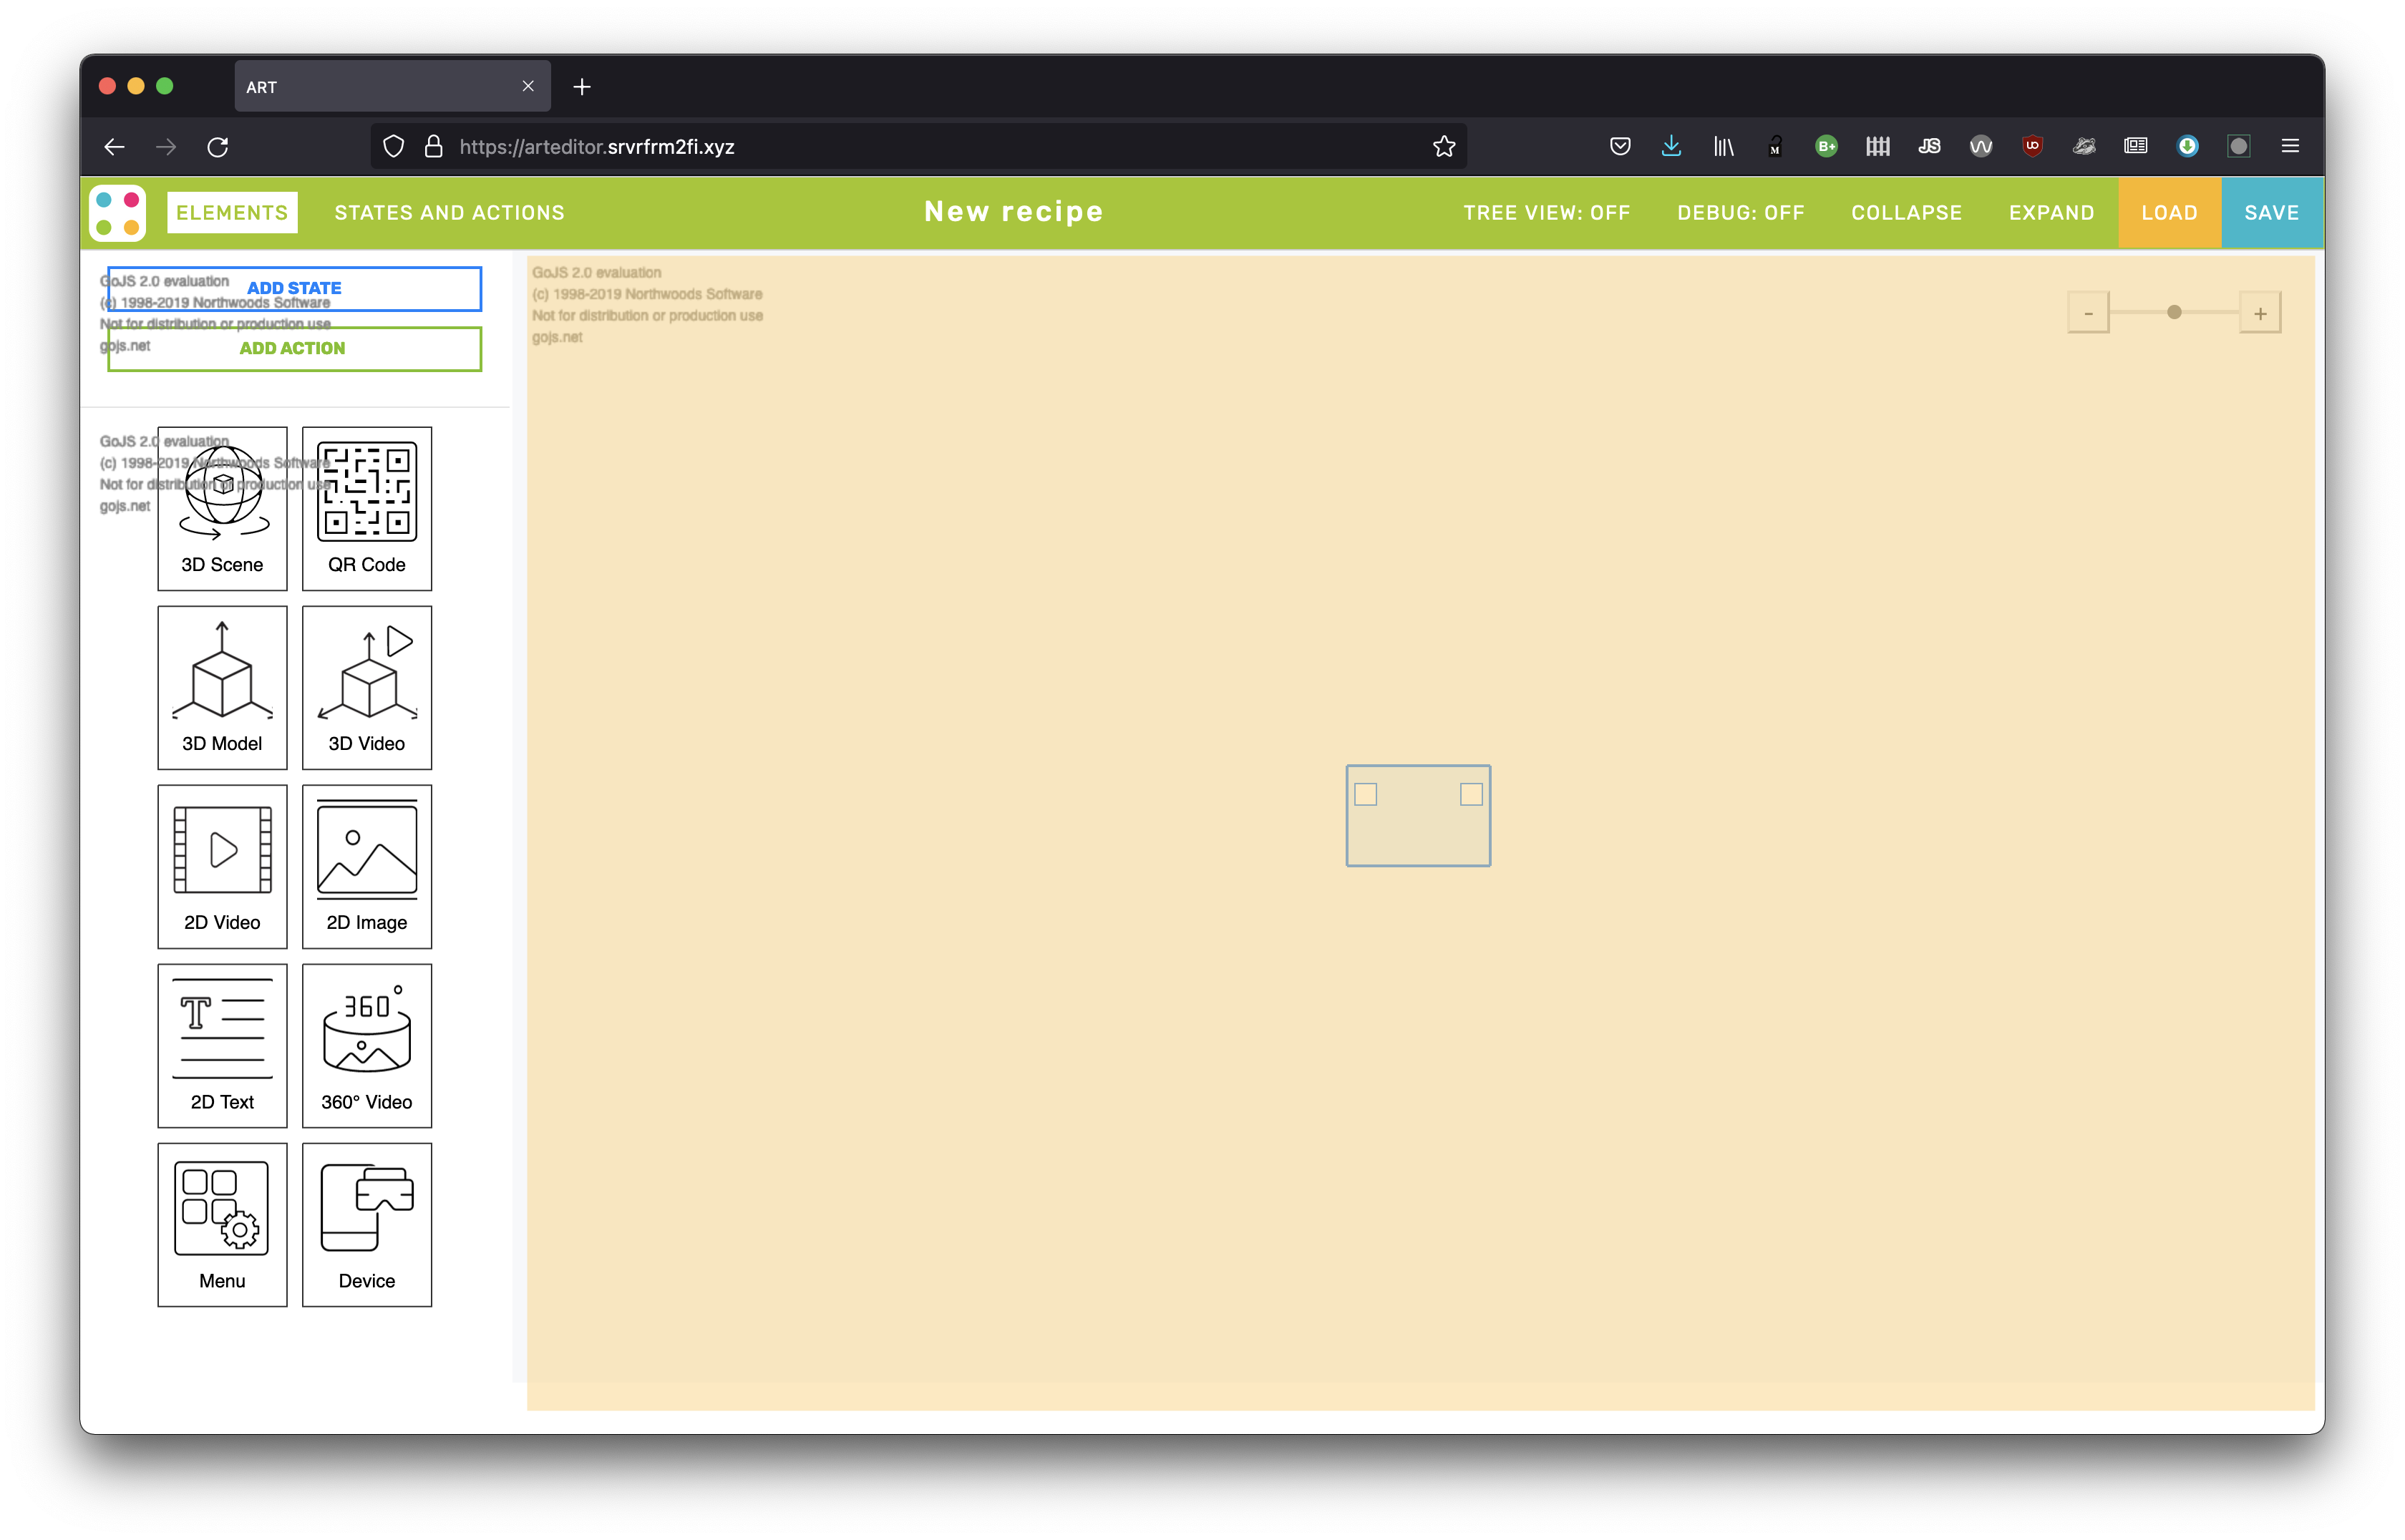
\includegraphics[width=\textwidth]{Figures/Editor/editor-ui-diagram.png}
    \caption{ART Editor GUI - Diagram}
    \label{fig:editor-ui-diagram}
\end{figure}

\begin{figure}[h]
    \centering
    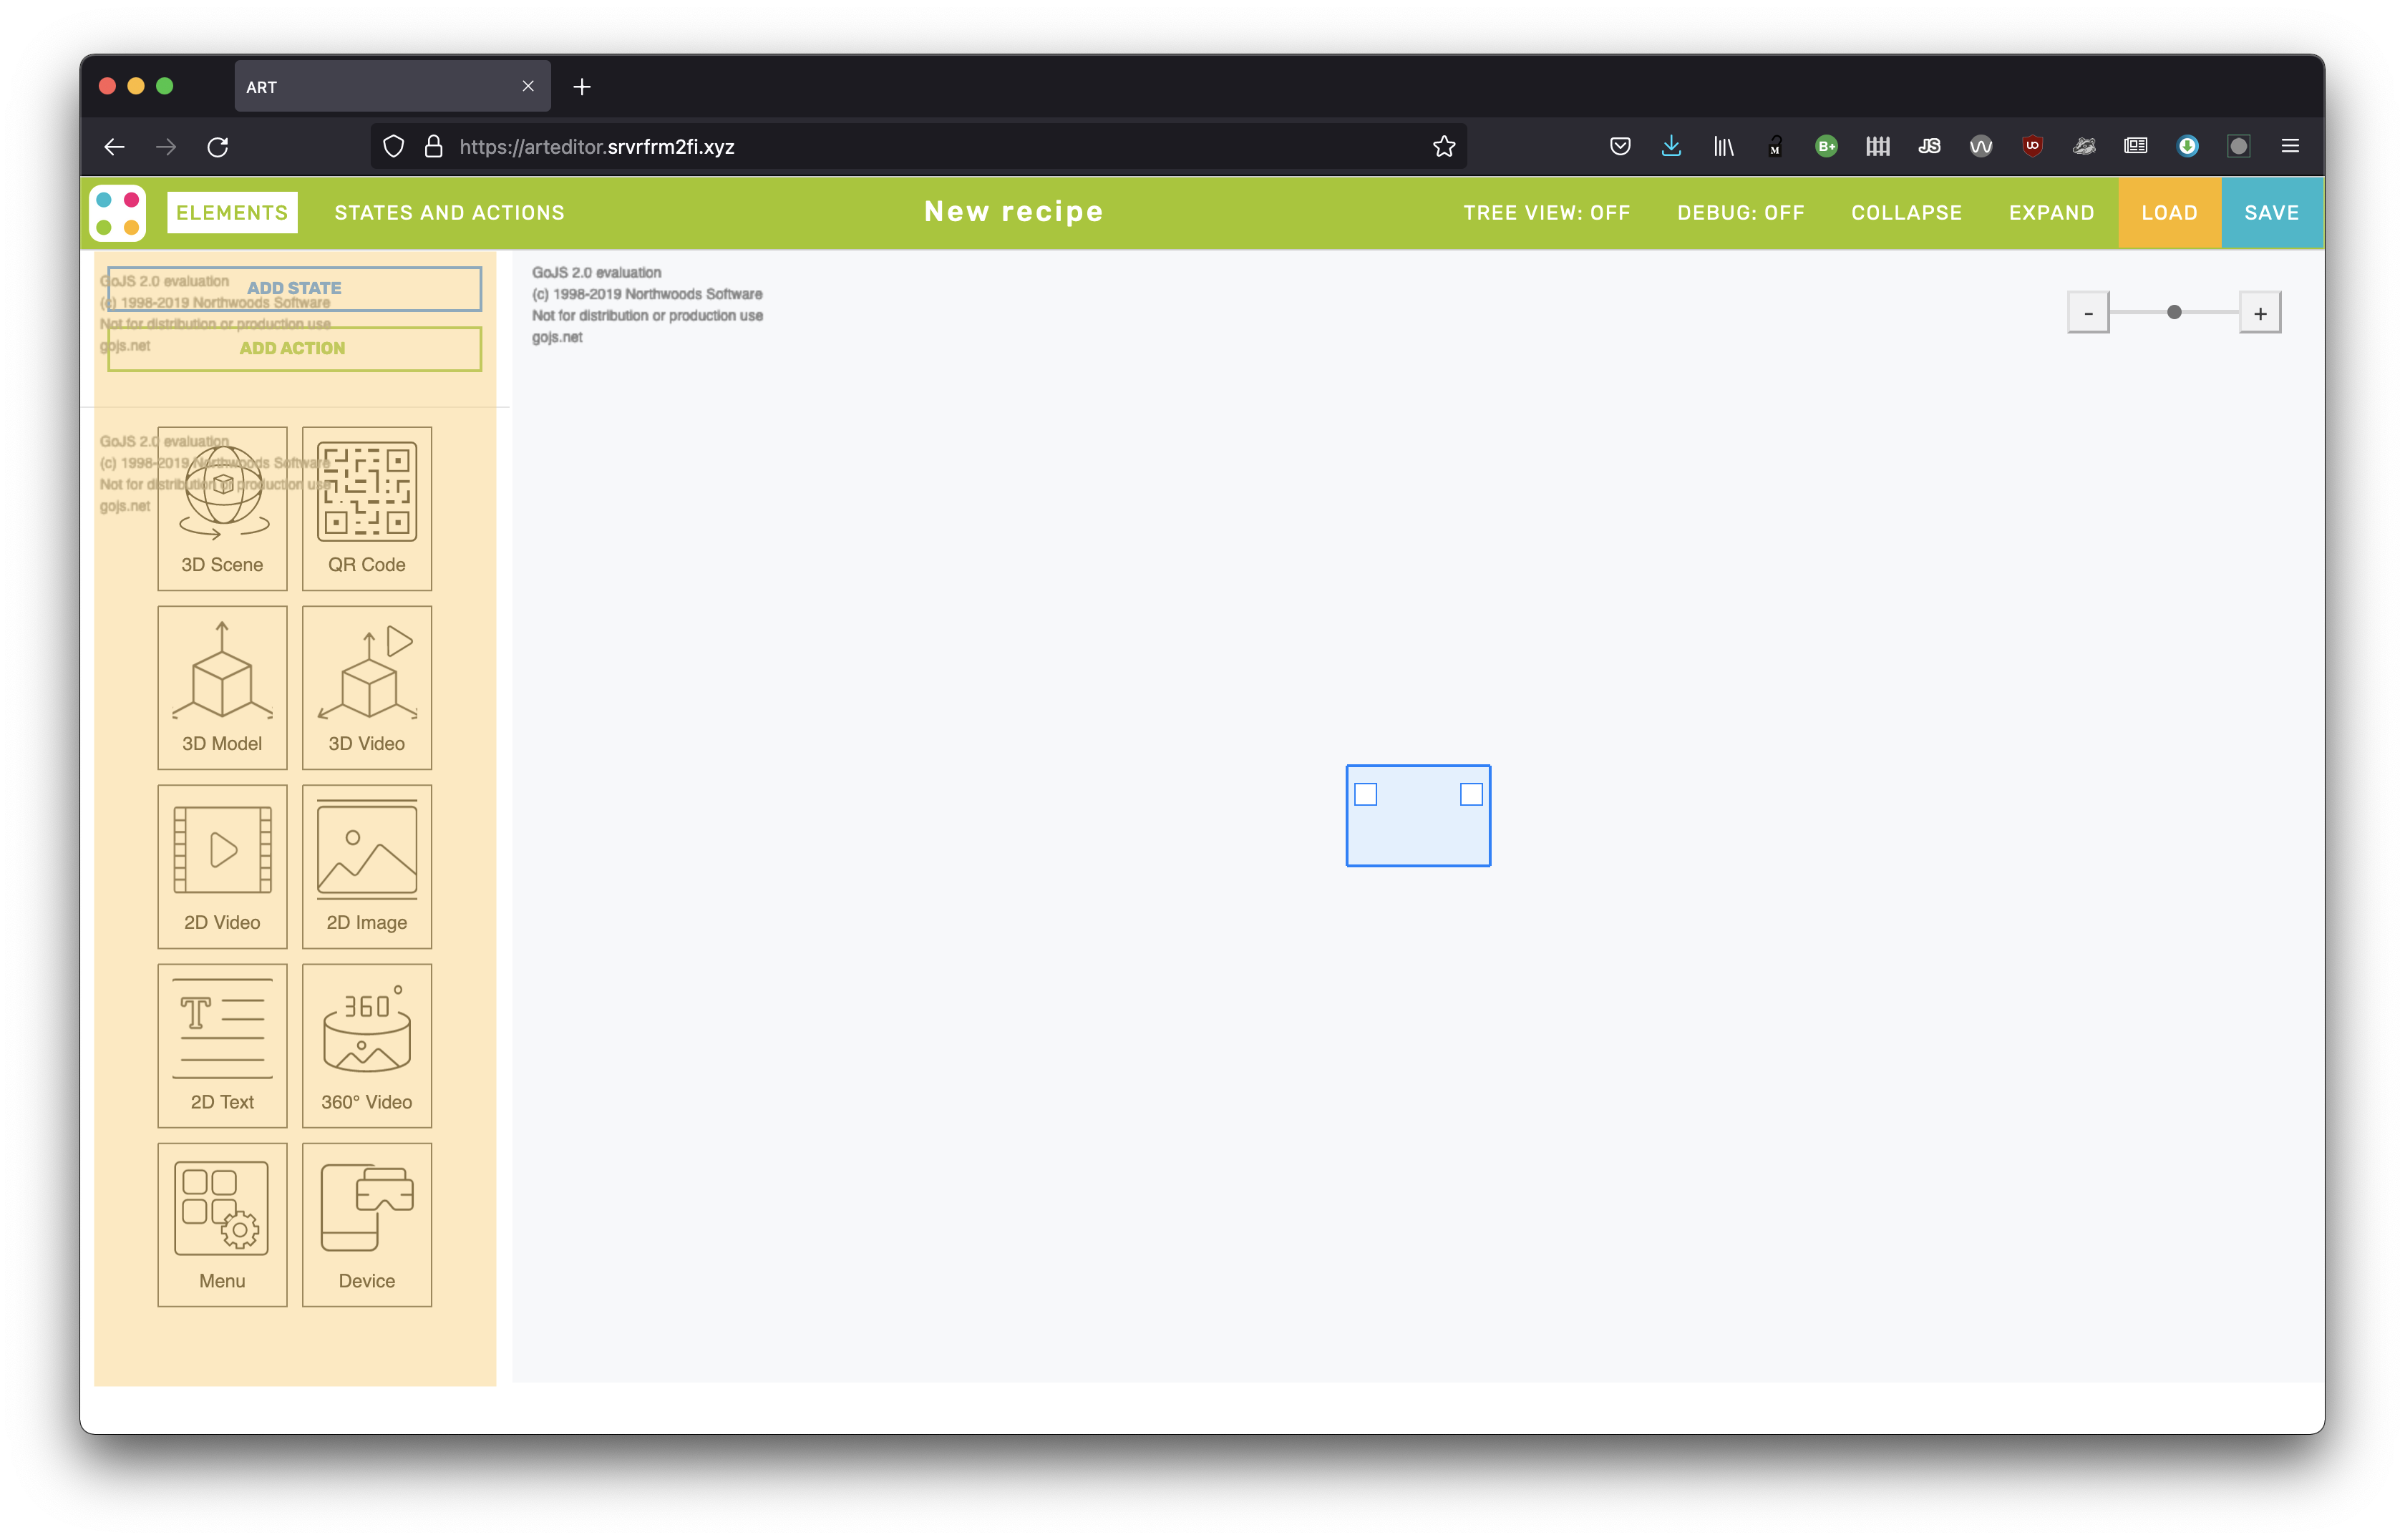
\includegraphics[width=\textwidth]{Figures/Editor/editor-ui-tab.png}
    \caption{ART Editor GUI - Left Paned Window}
    \label{fig:editor-ui-tab}
\end{figure}
On top of them a tab bar (\autoref{fig:editor-ui-topbar}) allows to switch between the elements and tags view, change the title and description of the diagram (by default called 'New Recipe') and load or save the \gls{JSON} configuration file.
\begin{figure}[H]
    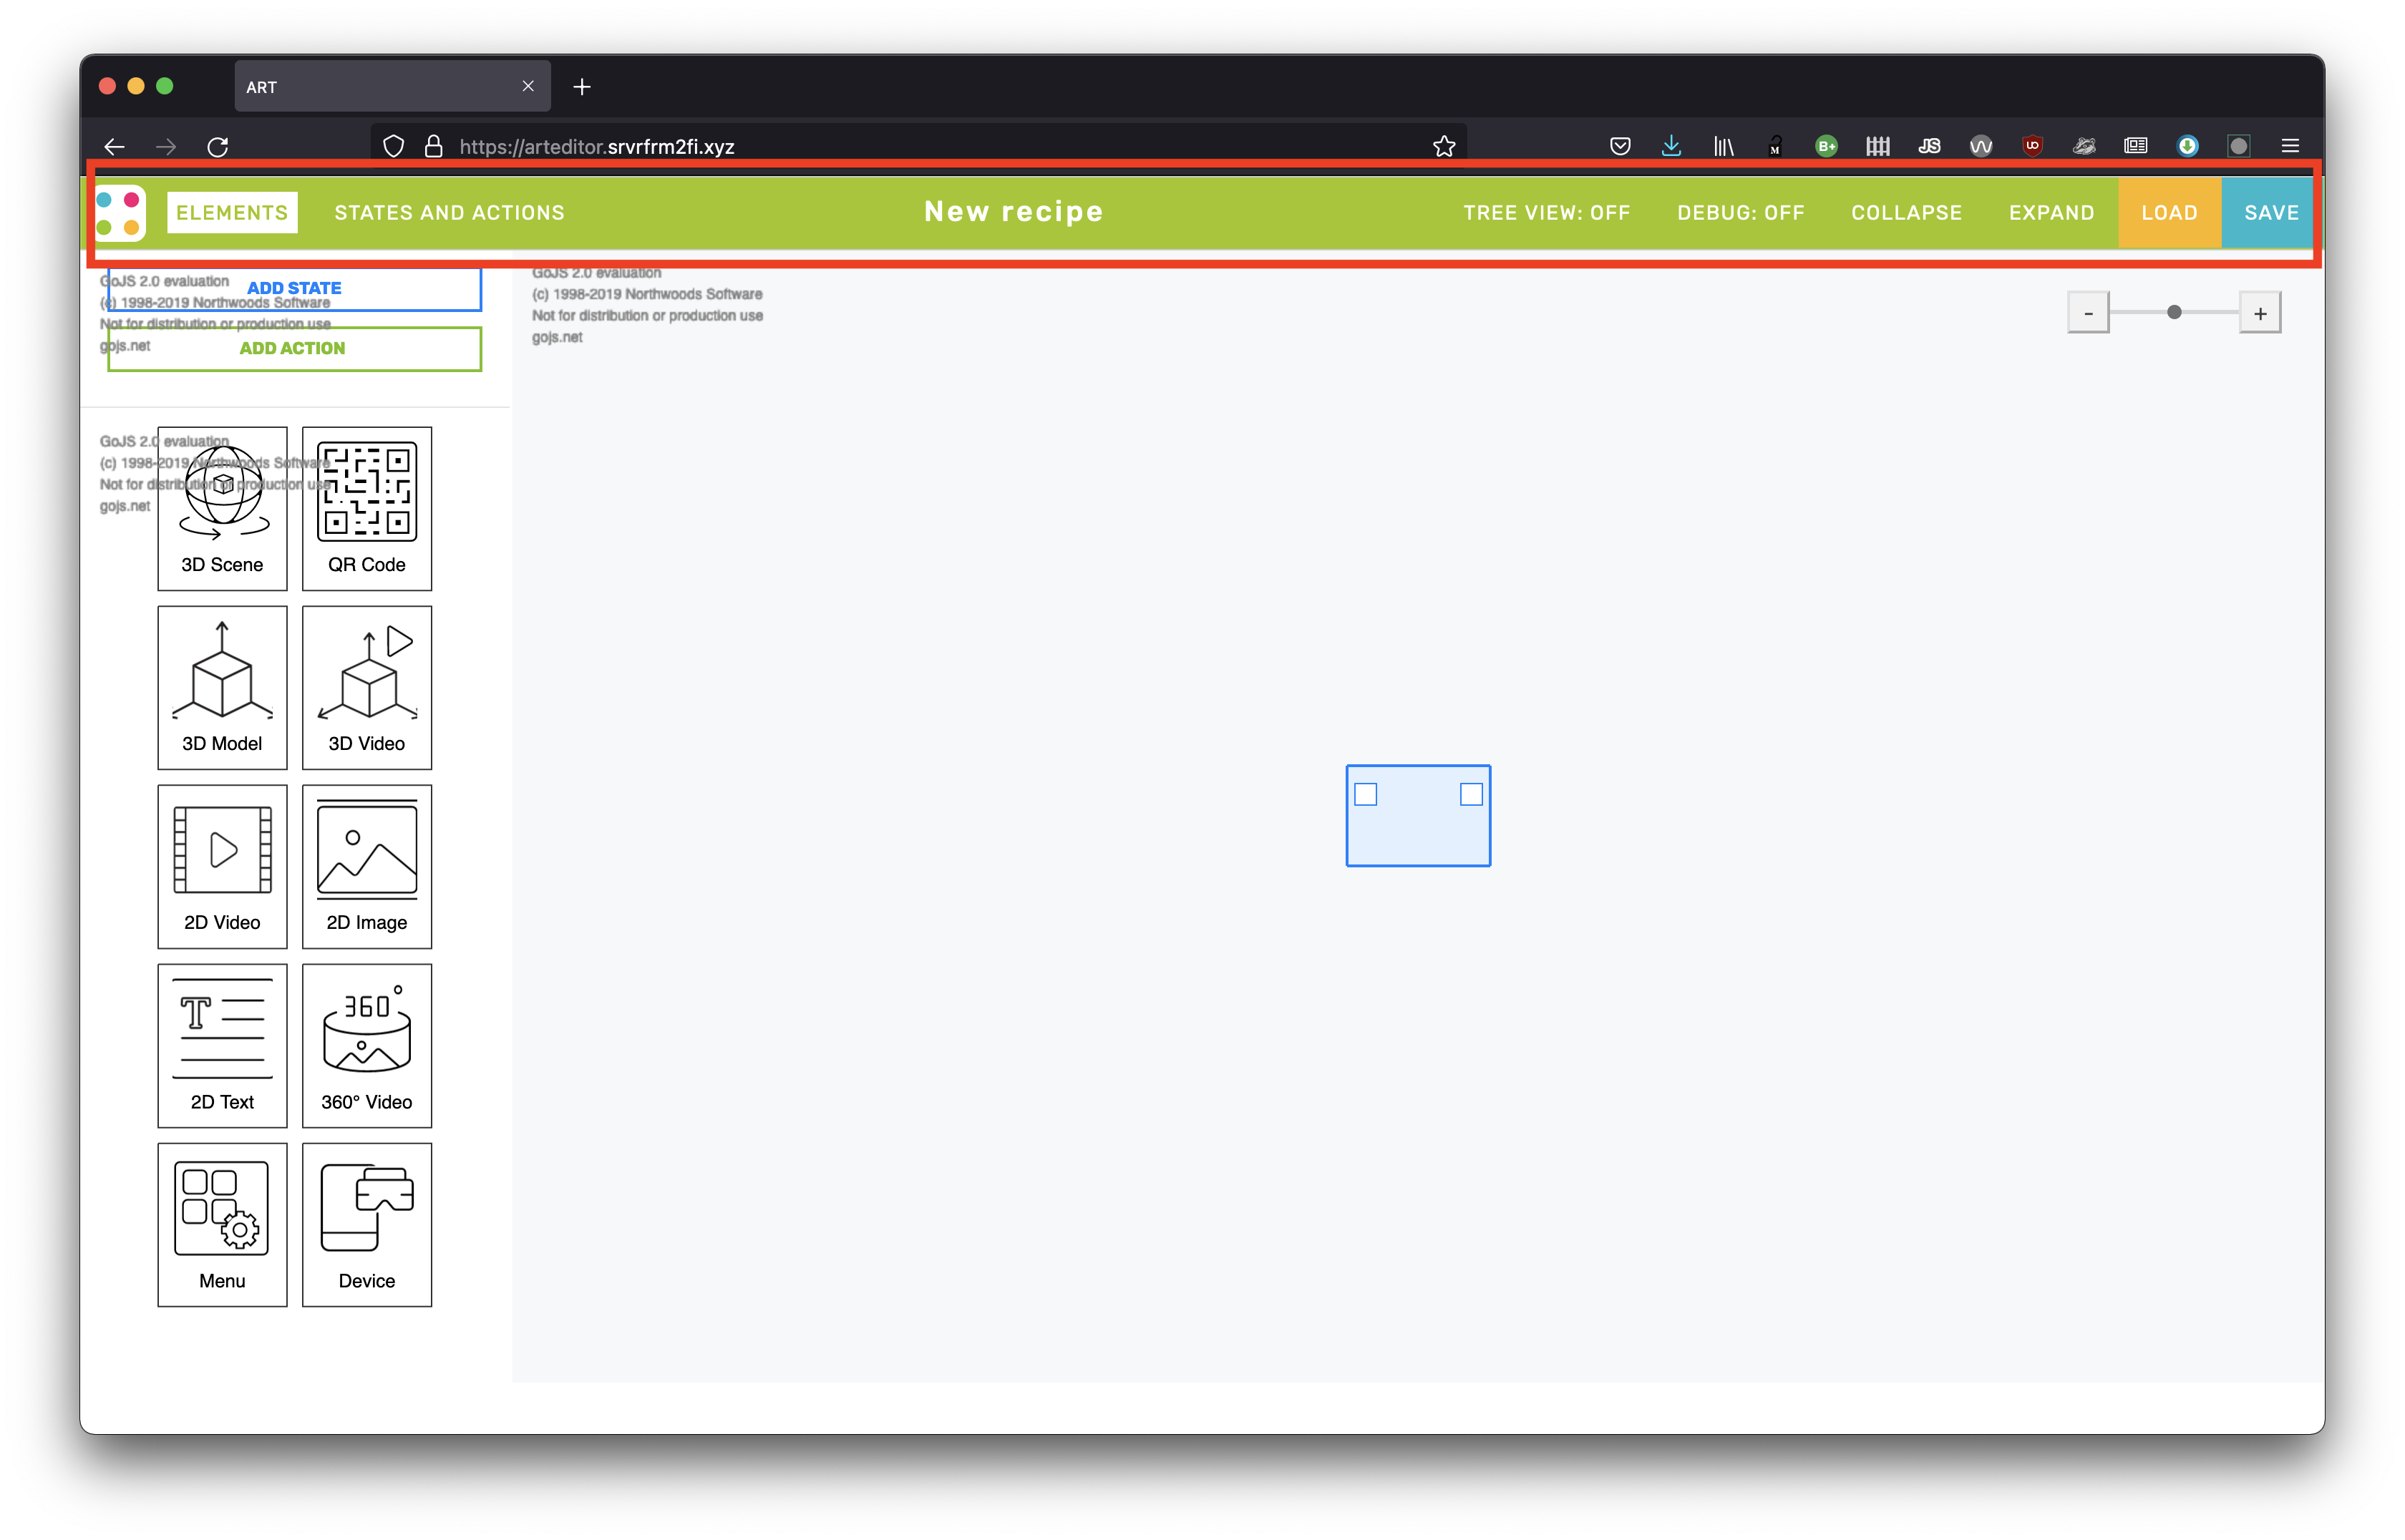
\includegraphics[width=\textwidth]{Figures/Editor/editor-ui-topbar.png}
    \caption{ART Editor GUI - Top Bar}
    \label{fig:editor-ui-topbar}
\end{figure}

Concerning the elements available to the editor, placeholder icons have been designed (\autoref{fig:art-editor-elements-icons}) in order to distinguish and move them onto the diagram, inside state and action nodes. Each time an element is dropped into a node the editor creates a new instance of that element, assigning a unique identifier (ID) on the upper-left corner of it (see \autoref{fig:art-effect}). It is then possible to change the label name of the element or, from the property inspector pane (\autoref{fig:property-inspector}), refer to an already existing element using its ID and, consequently, its name.
\begin{figure}[htbp]
    \hfill
    \begin{subfigure}{0.18\textwidth}
        \includesvg[width=\columnwidth,height=\columnwidth]{Figures/Editor/elements/3D-scene.svg}
        \caption{3D Scene}
    \end{subfigure}
    \hfill
    \begin{subfigure}{0.18\textwidth}
        \includesvg[width=\columnwidth,height=\columnwidth]{Figures/Editor/elements/3D-model.svg}
        \caption{3D Model}
    \end{subfigure}
    \hfill
    \begin{subfigure}{0.18\textwidth}
        \includesvg[width=\columnwidth,height=\columnwidth]{Figures/Editor/elements/3D-video.svg}
        \caption{3D Video}
    \end{subfigure}
    \hfill
    \begin{subfigure}{0.18\textwidth}
        \includesvg[width=\columnwidth,height=\columnwidth]{Figures/Editor/elements/2D-video.svg}
        \caption{2D Video}
    \end{subfigure}
    \hfill
    \begin{subfigure}{0.18\textwidth}
        \includesvg[width=\columnwidth,height=\columnwidth]{Figures/Editor/elements/2D-image.svg}
        \caption{2D Image}
    \end{subfigure}
    \hfill
    \begin{subfigure}{0.18\textwidth}
        \includesvg[width=\columnwidth,height=\columnwidth]{Figures/Editor/elements/2D-text.svg}
        \caption{2D Text}
    \end{subfigure}
    \hfill
    \begin{subfigure}{0.18\textwidth}
        \includesvg[width=\columnwidth,height=\columnwidth]{Figures/Editor/elements/qr-code.svg}
        \caption{QR Code}
    \end{subfigure}
    \hfill
    \begin{subfigure}{0.18\textwidth}
        \includesvg[width=\columnwidth,height=\columnwidth]{Figures/Editor/elements/360video.svg}
        \caption{360° Video}
    \end{subfigure}
    \hfill
    \begin{subfigure}{0.18\textwidth}
        \includesvg[width=\columnwidth,height=\columnwidth]{Figures/Editor/elements/menu.svg}
        \caption{Menu}
    \end{subfigure}
    \hfill
    \begin{subfigure}{0.18\textwidth}
        \includesvg[width=\columnwidth,height=\columnwidth]{Figures/Editor/elements/device.svg}
        \caption{Device}
    \end{subfigure}
    \hfill
    \caption{ART Editor's Element Icons}
    \label{fig:art-editor-elements-icons}
\end{figure}
\begin{figure}[H]
    \centering
    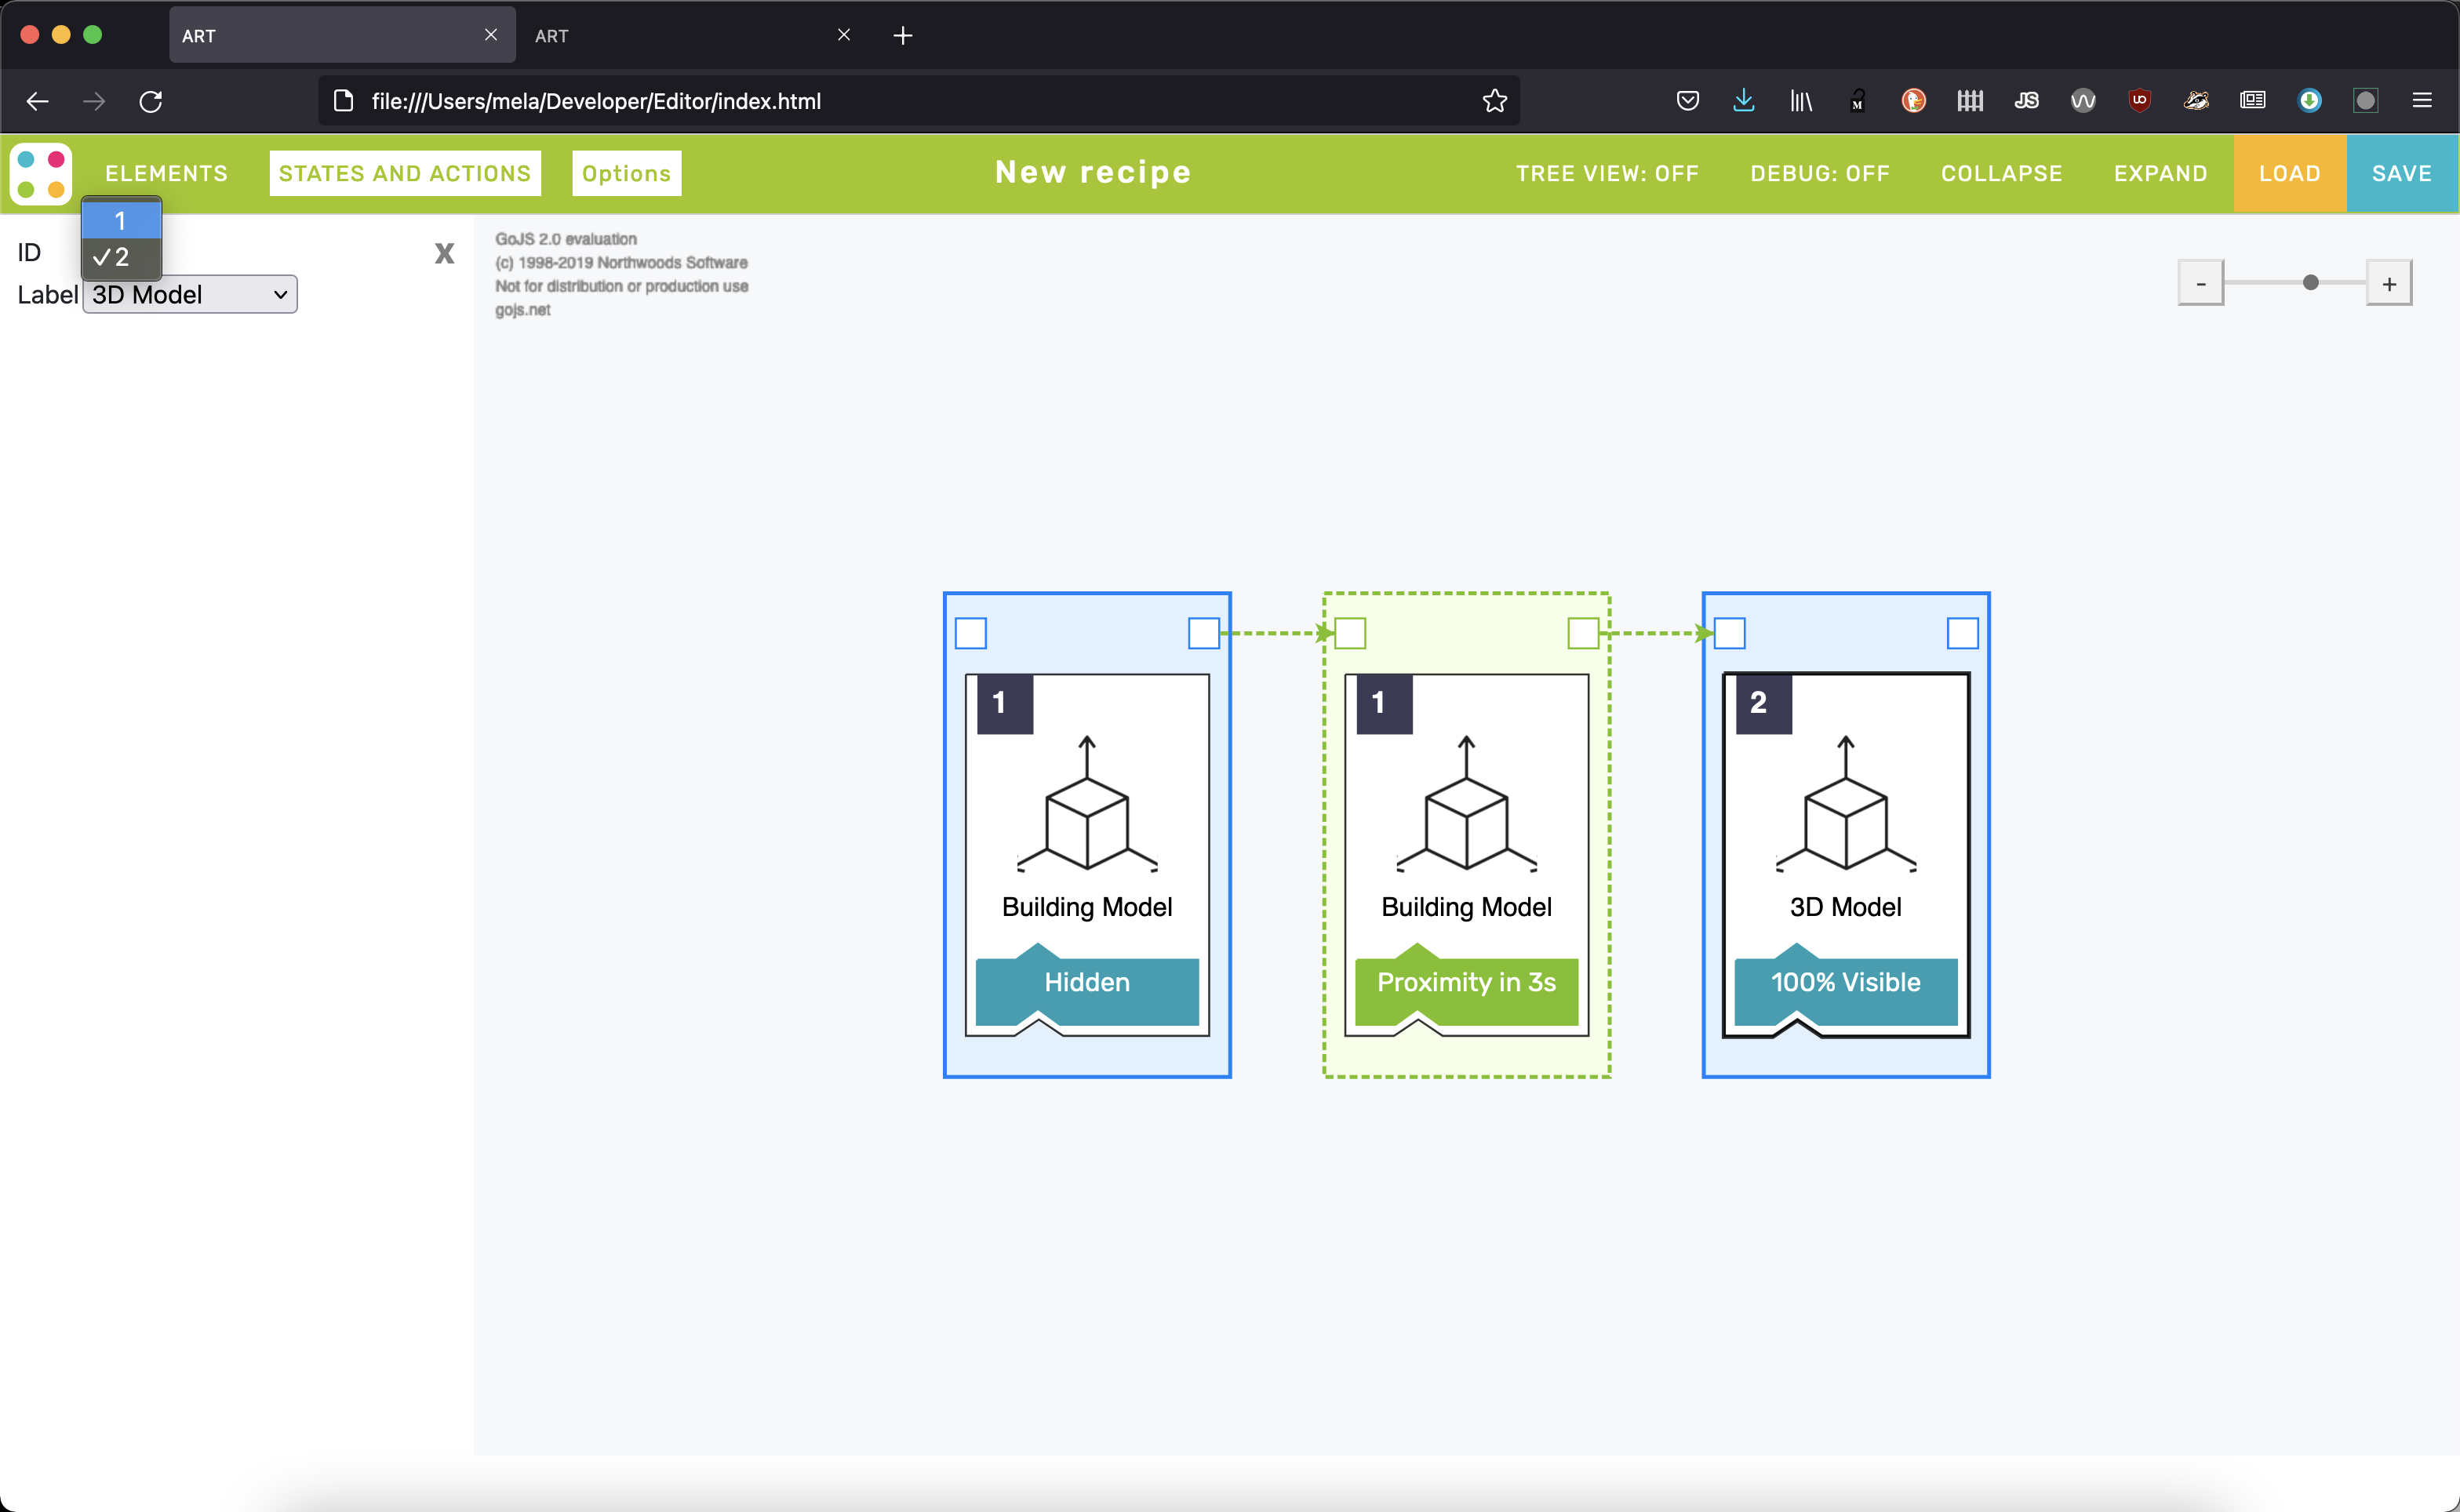
\includegraphics[width=\columnwidth]{Figures/Editor/element-inspector.png}
    \caption{Change of a 3D Model's ID and label from the elements property inspector pane}
    \label{fig:property-inspector}
\end{figure}

State and action nodes have a very clean UI easy to distinguish thanks to different colours used to represent them (\autoref{fig:state}, \autoref{fig:action}); nodes dimensions are responsive and automatically resize to fit their contents.
\begin{figure}[h]
    \begin{subfigure}{0.5\textwidth}
        \centering
        
\includegraphics{Figures/Editor/state.png}
        \caption{State}
        \label{fig:state}
    \end{subfigure}
    \begin{subfigure}{0.5\textwidth}
        \centering
        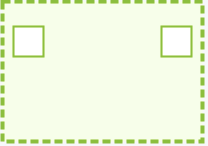
\includegraphics{Figures/Editor/action.png}
        \caption{Action}
        \label{fig:action}
    \end{subfigure}
    \caption{ART Editor Nodes}
\end{figure}
On the top left and right corners two squared boxes are used to draw -- by a click followed by drag-and-drop -- links between states and actions and vice versa, the former allowing multiple inputs (action nodes) while the latter only admits a final state. It has to be considered that multiple action nodes departing from the same state node describe a logical disjunction of events, while more elements with action tags inside an action node implement the logical conjunction. 

State and Action Tags, as well, have been designed for simplicity and usability, allowing an easily understandable drag-and-drop interaction modelling paradigm (\autoref{fig:state-tags}, \autoref{fig:action-tags}) onto their target elements.
\begin{figure}[h]
    \begin{subfigure}{0.4\textwidth}
        \centering
        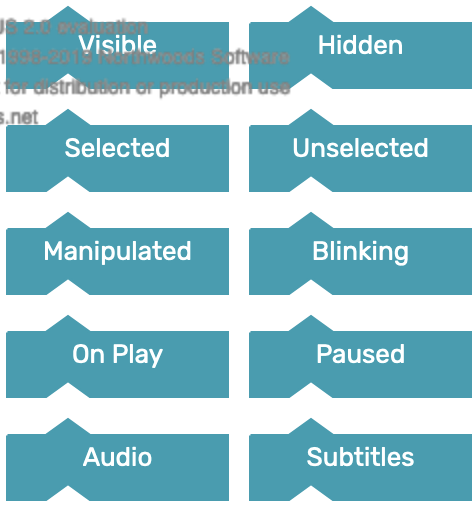
\includegraphics[width=\columnwidth]{Figures/Editor/state-tag.png}
        \caption{State Tags}
        \label{fig:state-tags}
    \end{subfigure}
    \hfill
    \begin{subfigure}{0.4\textwidth}
        \centering
        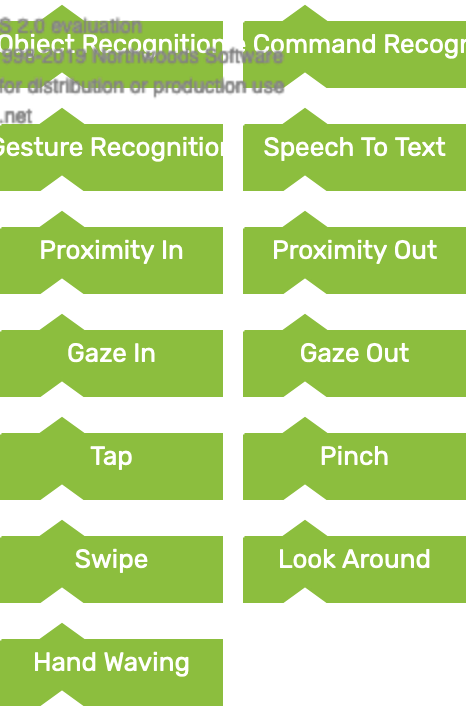
\includegraphics[width=\columnwidth]{Figures/Editor/action-tag.png}
        \caption{Action Tags}
        \label{fig:action-tags}
    \end{subfigure}
    \caption{ART Editor Tags}
\end{figure}
